% Options for packages loaded elsewhere
\PassOptionsToPackage{unicode}{hyperref}
\PassOptionsToPackage{hyphens}{url}
\PassOptionsToPackage{dvipsnames,svgnames*,x11names*}{xcolor}
%
\documentclass[
]{article}
\usepackage{amsmath,amssymb}
\usepackage{lmodern}
\usepackage{ifxetex,ifluatex}
\ifnum 0\ifxetex 1\fi\ifluatex 1\fi=0 % if pdftex
  \usepackage[T1]{fontenc}
  \usepackage[utf8]{inputenc}
  \usepackage{textcomp} % provide euro and other symbols
\else % if luatex or xetex
  \usepackage{unicode-math}
  \defaultfontfeatures{Scale=MatchLowercase}
  \defaultfontfeatures[\rmfamily]{Ligatures=TeX,Scale=1}
\fi
% Use upquote if available, for straight quotes in verbatim environments
\IfFileExists{upquote.sty}{\usepackage{upquote}}{}
\IfFileExists{microtype.sty}{% use microtype if available
  \usepackage[]{microtype}
  \UseMicrotypeSet[protrusion]{basicmath} % disable protrusion for tt fonts
}{}
\makeatletter
\@ifundefined{KOMAClassName}{% if non-KOMA class
  \IfFileExists{parskip.sty}{%
    \usepackage{parskip}
  }{% else
    \setlength{\parindent}{0pt}
    \setlength{\parskip}{6pt plus 2pt minus 1pt}}
}{% if KOMA class
  \KOMAoptions{parskip=half}}
\makeatother
\usepackage{xcolor}
\IfFileExists{xurl.sty}{\usepackage{xurl}}{} % add URL line breaks if available
\IfFileExists{bookmark.sty}{\usepackage{bookmark}}{\usepackage{hyperref}}
\hypersetup{
  pdftitle={Lab 02},
  pdfauthor={Dr.~Patrick Bitterman},
  colorlinks=true,
  linkcolor=Maroon,
  filecolor=Maroon,
  citecolor=Blue,
  urlcolor=Blue,
  pdfcreator={LaTeX via pandoc}}
\urlstyle{same} % disable monospaced font for URLs
\usepackage[margin=1in]{geometry}
\usepackage{graphicx}
\makeatletter
\def\maxwidth{\ifdim\Gin@nat@width>\linewidth\linewidth\else\Gin@nat@width\fi}
\def\maxheight{\ifdim\Gin@nat@height>\textheight\textheight\else\Gin@nat@height\fi}
\makeatother
% Scale images if necessary, so that they will not overflow the page
% margins by default, and it is still possible to overwrite the defaults
% using explicit options in \includegraphics[width, height, ...]{}
\setkeys{Gin}{width=\maxwidth,height=\maxheight,keepaspectratio}
% Set default figure placement to htbp
\makeatletter
\def\fps@figure{htbp}
\makeatother
\setlength{\emergencystretch}{3em} % prevent overfull lines
\providecommand{\tightlist}{%
  \setlength{\itemsep}{0pt}\setlength{\parskip}{0pt}}
\setcounter{secnumdepth}{-\maxdimen} % remove section numbering
\ifluatex
  \usepackage{selnolig}  % disable illegal ligatures
\fi

\title{Lab 02}
\author{Dr.~Patrick Bitterman}
\date{}

\begin{document}
\maketitle

\hypertarget{lab-02-geoprocessing-in-arcgis-pro}{%
\section{Lab 02: Geoprocessing in ArcGIS
Pro}\label{lab-02-geoprocessing-in-arcgis-pro}}

\hypertarget{read-the-instructions-completely-before-starting-the-lab}{%
\subsubsection{Read the instructions COMPLETELY before starting the
lab}\label{read-the-instructions-completely-before-starting-the-lab}}

\hypertarget{part-1-an-example-of-geoprocessing-using-python-and-some-arcgis-pro}{%
\subsection{Part 1: An example of geoprocessing using Python (and some
ArcGIS
Pro)}\label{part-1-an-example-of-geoprocessing-using-python-and-some-arcgis-pro}}

Part 1 will familiarize you with some functions we have discussed by not
yet used in class.

\begin{enumerate}
\def\labelenumi{\arabic{enumi}.}
\tightlist
\item
  Download and extract the \texttt{lab02data.zip} file from the course
  GitHub respository to a sensible location on your computer. For the
  purposes of these examples, I will assume your workspace is setup as:
\end{enumerate}

\begin{verbatim}
arcpy.env.workspace = "C://GEOG432//lab02//"
\end{verbatim}

However, you may use whatever workspace location you choose.

\begin{enumerate}
\def\labelenumi{\arabic{enumi}.}
\tightlist
\item
  Run the following code:
\end{enumerate}

\begin{verbatim}
arcpy.Exists("hospitals.shp")
\end{verbatim}

The result is True.

The \textbf{Exists()} function returns a Boolean value. Several other
ArcPy functions also are not geoprocessing tools, and some of them are
used later in this exercise and others.

The \textbf{Usage()} function is a useful shortcut for getting the
syntax of ArcPy functions without relying on the pop-ups in the Python
windows.

\begin{enumerate}
\def\labelenumi{\arabic{enumi}.}
\setcounter{enumi}{1}
\tightlist
\item
  Run the following code:
\end{enumerate}

\begin{verbatim}
arcpy.Usage("Clip_analysis")
\end{verbatim}

The result is

\begin{verbatim}
'Clip_analysis(in_features, clip_features, out_feature_class, {cluster_tolerance})'
\end{verbatim}

Remember to use a toolbox alias to call geoprocessing tools. Calling a
tool by name only will produce an error.

\begin{enumerate}
\def\labelenumi{\arabic{enumi}.}
\setcounter{enumi}{2}
\tightlist
\item
  Run the following code:
\end{enumerate}

\begin{verbatim}
arcpy.Usage("Clip")
\end{verbatim}

The result is

`Method Clip not found. Choices: Method Clip not found.'

The Usage function applies to all ArcPy functions, not only to
geoprocessing tools.

\begin{enumerate}
\def\labelenumi{\arabic{enumi}.}
\setcounter{enumi}{3}
\tightlist
\item
  Run the following code:
\end{enumerate}

\begin{verbatim}
arcpy.Usage("Exists")
\end{verbatim}

The result is

`exists(, \{datatype\}) -\textgreater{} boolean Check if a data element
exists.'

In addition to functions, ArcPy also contains several classes. Classes
are often used as shortcuts to complete tool parameters. You already
have become familiar with using the env class to set environment
properties. Another commonly used class is the SpatialReference class.

\begin{enumerate}
\def\labelenumi{\arabic{enumi}.}
\setcounter{enumi}{4}
\tightlist
\item
  In ArcGIS Pro, add hospitals.shp to a new map.
\end{enumerate}

The spatial reference of this shapefile is missing. As a result, the
hospitals show up in northern Finland instead of Austin, Texas. This
happens because the coordinates are displayed in the default Web
Mercator coordinate system.

\begin{figure}
\centering
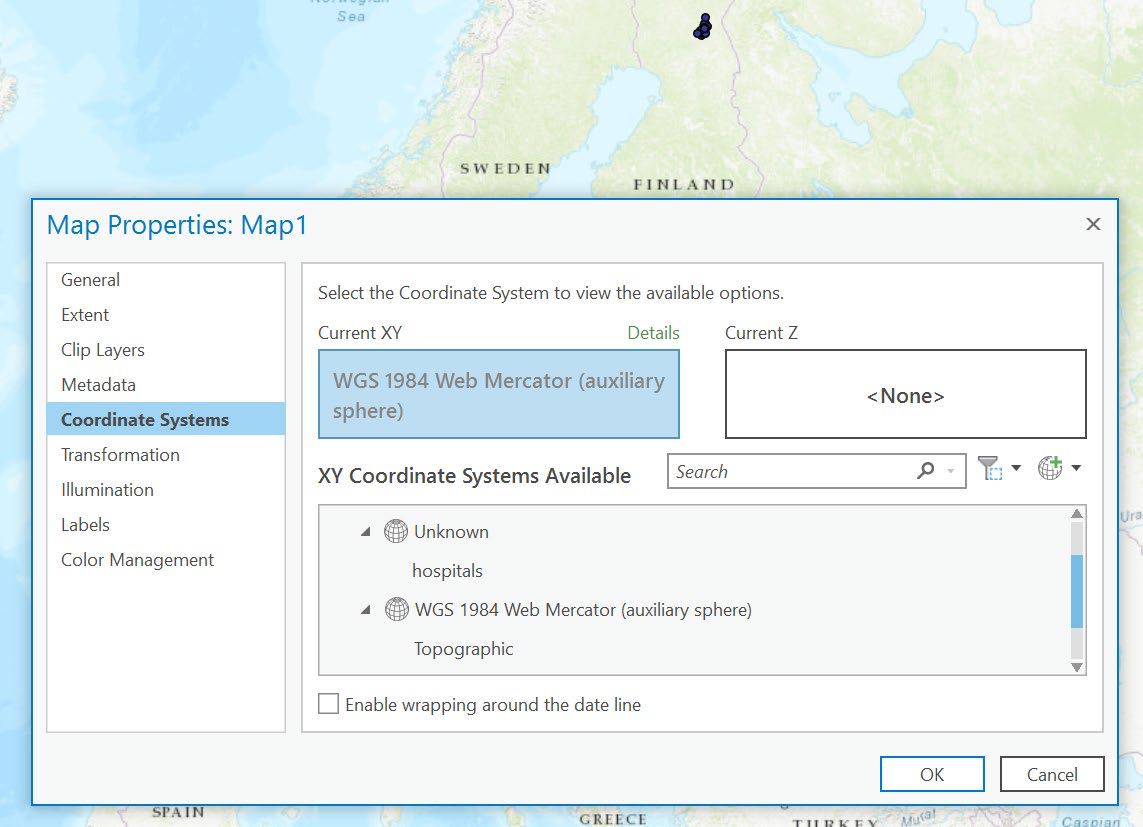
\includegraphics{../images/lab02_noproj.png}
\caption{No projection}
\end{figure}

You will use the Define Projection tool to fix it. The syntax of the
Define Projection tool is as follows:

\begin{verbatim}
DefineProjection_management(in_dataset, coor_system)
\end{verbatim}

\begin{enumerate}
\def\labelenumi{\arabic{enumi}.}
\setcounter{enumi}{5}
\tightlist
\item
  Run the following code: (note, your files may be in a different
  location)
\end{enumerate}

\begin{verbatim}
prjfile = "C:\\GEOG432\\lab02\\facilities.prj"

spatial_ref = arcpy.SpatialReference(prjfile)
\end{verbatim}

This spatial reference object can now be used for other purposes.

\begin{enumerate}
\def\labelenumi{\arabic{enumi}.}
\setcounter{enumi}{6}
\tightlist
\item
  Run the following code:
\end{enumerate}

\begin{verbatim}
arcpy.DefineProjection_management("hospitals", spatial_ref) 
\end{verbatim}

The result is: \textbf{\textless Result `hospitals'\textgreater{}}

The SpatialReference object is used in the Define Projection tool to
specify the coordinate system of the hospitals.shp file. In this
example, the coordinate system parameter also could be specified by
directly referencing the .prj file as a parameter of the Define
Projection tool. However, creating a spatial reference object also gives
you access to its many properties.

\begin{enumerate}
\def\labelenumi{\arabic{enumi}.}
\setcounter{enumi}{7}
\tightlist
\item
  Run the following code:
\end{enumerate}

\begin{verbatim}
print(spatial_ref.name)
\end{verbatim}

The result is

\textbf{NAD\_1983\_StatePlane\_Texas\_Central\_FIPS\_4203\_Feet.}

\begin{enumerate}
\def\labelenumi{\arabic{enumi}.}
\setcounter{enumi}{8}
\tightlist
\item
  Run the following code:
\end{enumerate}

\begin{verbatim}
print(spatial_ref.linearUnitName)
\end{verbatim}

The result is

Foot\_US.

\begin{enumerate}
\def\labelenumi{\arabic{enumi}.}
\setcounter{enumi}{9}
\tightlist
\item
  Run the following code:
\end{enumerate}

\begin{verbatim}
print(spatial_ref.XYResolution)
\end{verbatim}

The result is

0.000328083333333.

The result of running the Define Project tool is that the feature class
hospitals.shp is assigned the correct coordinate system.

\begin{enumerate}
\def\labelenumi{\arabic{enumi}.}
\setcounter{enumi}{10}
\tightlist
\item
  Right-click on the hospitals data layer in the Content panel of the
  active map, and click Zoom To Layer.
\end{enumerate}

The hospitals are now showing where they belong---i.e., in Austin,
Texas.

\begin{figure}
\centering
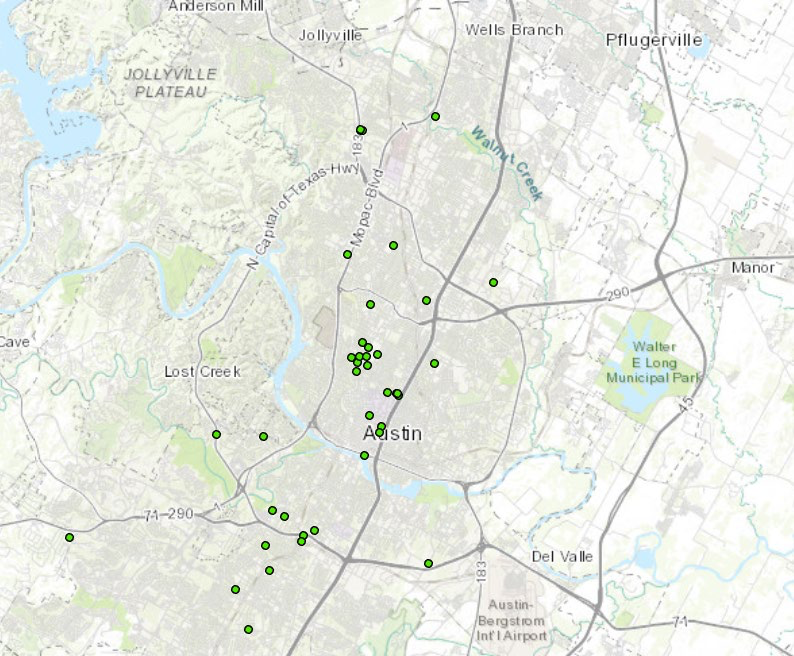
\includegraphics{../images/lab02_intexas.png}
\caption{in Texas}
\end{figure}

\newpage

\hypertarget{part-2-some-simple-analysis-on-your-own}{%
\subsection{Part 2: Some simple analysis on your
own}\label{part-2-some-simple-analysis-on-your-own}}

Often when we produce analysis, we rely on other tools (e.g., data
visualization, statistical software) \textbf{in addition to} our
geoprocessing workflows. For this part of the lab, you will be tasked to
complete a simple analysis of distance in Vermont.

\hypertarget{your-data}{%
\subsubsection{Your data:}\label{your-data}}

\begin{itemize}
\item
  vt\_munis.shp: a feature class that contains all of the Vermont
  municipalities (i.e., towns, cities, and villages) that intersect the
  Lake Champlain Basin
\item
  lake\_champlain.shp: a feature class of Lake Champlain
\end{itemize}

\hypertarget{your-tasks}{%
\subsubsection{Your tasks:}\label{your-tasks}}

\begin{enumerate}
\def\labelenumi{\arabic{enumi}.}
\tightlist
\item
  Write a Python script (using arcpy) that calculates the distance FROM
  ALL municipalities TO Lake Champlain
\item
  Create a map (using the ArcGIS Pro GUI) that symbolizes that distance
  in a meaningful way. This will serve as a quick check that you have
  successfully calculated distance
\item
  Produce a histogram that plots the distribution of distance values.
  You may use any tool you like (e.g., R, Excel, something from the web)
\item
  Using arcpy, reproject the \emph{vt\_munis} feature class (whatever
  projection you wish), \textbf{then recalculate distance(s) to Lake
  Champlain}
\item
  Finally, \textbf{for each municipality}, calculate the
  \emph{differences} between the 2 distances and report using summary
  statistics (mean, median, standard deviation)
\item
  Answer the questions below
\end{enumerate}

\newpage

\hypertarget{part-3-building-a-model-with-python}{%
\subsection{Part 3: building a model with
Python}\label{part-3-building-a-model-with-python}}

In lab 1 (part 2), you completed the following:

\begin{enumerate}
\def\labelenumi{\arabic{enumi}.}
\tightlist
\item
  Interpolated a precipitation surface from your points
\item
  Reclassifed the interpolated surface into an ordinal classification of
  precipitation ``zones'' that delineate relatively dry, medium, and wet
  regions
\item
  Created vector polygons from the zones
\item
  Clippe the zone polygons to the boundary of Nebraska
\end{enumerate}

\hypertarget{todays-task-replicate-the-workflow-in-a-python-script}{%
\subsubsection{Today's task: replicate the workflow in a Python
script}\label{todays-task-replicate-the-workflow-in-a-python-script}}

\begin{enumerate}
\def\labelenumi{\arabic{enumi}.}
\tightlist
\item
  Replicate the workflow using Python (and arcPy) ONLY!
\item
  Then, export your model from Lab 1 as a Python Script
\item
  Compare the model-generated code to what you wrote. Answer the
  questions below:
\end{enumerate}

\newpage

\hypertarget{questions}{%
\subsection{Questions:}\label{questions}}

\hypertarget{part-2}{%
\subsubsection{Part 2:}\label{part-2}}

\begin{enumerate}
\def\labelenumi{\arabic{enumi}.}
\tightlist
\item
  How is distance defined in your calculation?
\item
  What control do you have over the distance calculation?
\item
  How might alternative conceptualizations of ``distance'' affect the
  analysis? (note, for this question I am NOT referring to differences
  in projection or CRS)
\item
  What coordinate reference system (CRS) was vt\_munis originally in?
  What CRS did you change it to?
\item
  How did the calculation of distance change after you reprojected?
\end{enumerate}

\hypertarget{part-3}{%
\subsubsection{Part 3:}\label{part-3}}

\begin{enumerate}
\def\labelenumi{\arabic{enumi}.}
\setcounter{enumi}{5}
\tightlist
\item
  What challenges did you encounter in writing your script to accomplish
  the task? How did you overcome them?
\item
  How did the model-generated code differ to what you wrote? Would you
  now do anything differently? (note, just because it was created by
  ArcGIS Pro, doesn't mean it's the absolute best way to accomplish the
  task)
\end{enumerate}

\hypertarget{what-to-turn-in}{%
\subsection{What to turn in:}\label{what-to-turn-in}}

\begin{itemize}
\tightlist
\item
  Answers to the questions above
\item
  Map from part 2
\item
  Histogram from part 2
\item
  Summary statistics from part 2
\item
  Script from part 2
\item
  Script from part 3
\end{itemize}

\end{document}
